% Author: Till Tantau
% Source: The PGF/TikZ manual
\documentclass{minimal}

\usepackage{tikz}
\usetikzlibrary{trees,snakes}
\begin{document}
\pagestyle{empty}
\tikzstyle{level 1}=[sibling angle=120]
\tikzstyle{level 2}=[sibling angle=60]
\tikzstyle{level 3}=[sibling angle=75]
\tikzstyle{level 4}=[sibling angle=75]
\tikzstyle{every node}=[fill]
\tikzstyle{edge from parent}=[snake=expanding waves,segment length=1mm,
                              segment angle=10,draw]
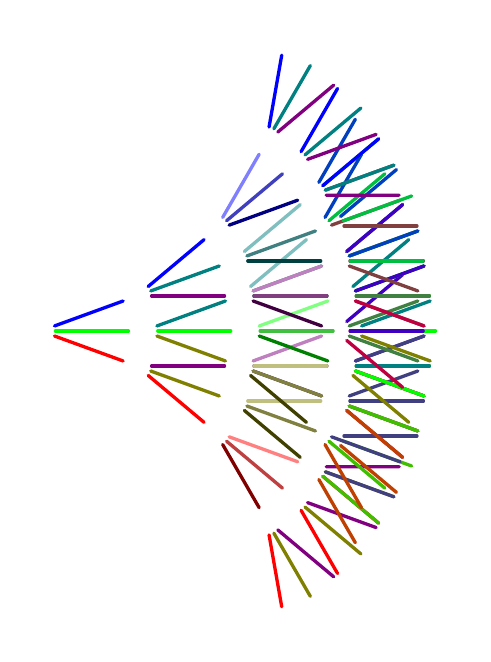
\begin{tikzpicture}[grow cyclic,shape=circle,very thick,level distance=13mm,
                    cap=round]
\node {} child [color=\A] foreach \A in {red,green,blue}
    { node {} child [color=\A!50!\B] foreach \B in {red,green,blue}
        { node {} child [color=\A!50!\B!50!\C] foreach \C in {black,gray,white}
            { node {} child [color=\A!50!\B!50!\C] foreach \C in {red,green,blue}
                    { node {} }
            }
        }
    };
\end{tikzpicture}

\end{document}

